\documentclass{article}
\usepackage{amsmath}
\usepackage{mathtools}
\usepackage{graphicx, color}
\graphicspath{{figs/}}

%----------------------------------
%\topmargin      -1.5cm   % read Lamport p.163
%\oddsidemargin  -0.04cm  % read Lamport p.163
%\evensidemargin -0.04cm  % same as oddsidemargin but for left-hand pages
%\textwidth      16.59cm
%\textheight     22.94cm

\topmargin      -1.5cm   % read Lamport p.163
\oddsidemargin  0.04cm  % read Lamport p.163
\evensidemargin 0.04cm  % same as oddsidemargin but for left-hand pages
\textwidth      15cm
\textheight     22.94cm

\parskip         7.2pt   % sets spacing between paragraphs
\parindent         3mm   % sets leading space for paragraphs
%-------------------------------------
\title{ Modelling Birds Population }
\author{Ignacio Alvarez}
\date{ Fall 2013 }

\begin{document}
\maketitle 

\vspace{3cm}

\section{Introduction} 
According to (REF, Etterson) one of the basic research goals in Ecology consist on understand the distribution and abundance of the animal population. In this work, the particular goal will be to explore alternatives to model the time trends in Western Great Lakes Birds population over 1994 to 2011. 

\subsection{Data description}

The data source for this study came from ``an extensive, long-term monitoring program with over 1600 off-road sampling points designed to track regional population trends and investigate the response of forest birds to regional land use patterns''(REF:). 

This monitoring program is carry out by Natural Resources Research Institute (University of Minnesota Duluth) with the objective of ``sustain forest resources and bird diversity in western Great Lakes forests'' (REF: ). 

For this report in particular the dataset which will be used in this report consist in the yearly bird count for 73 species on three National Forest from 1995 to 2013. There are several interesting covariate that are relavated in the sampling procedure, however most of them are site characteristics at the moment when the sampling was done, therefore they are not so meaningfully when we consider yearly aggregated data.  

We can see a first look of the data in Figure \ref{figtr}, where the total bird count per year is plotted for all three forest. We can see Superior is consistently over all years the forest with more bird counts (why? is bigger ?) reaching 10000 counts on three time during the monitoring period. The others two forest, Chequamegon and Chippewa show a similar trend in the total bird count. 

Overall, it seems to be a first sub-period from 1995 to 2003 where the total bird count is increasing every year but from that this increment stop. From 2003 on Superior forest it seem to oscillate around a little more than 8000 birds while for Chequamegon the count are getting smaller each year. 

\begin{figure}[h!]
\centering
\includegraphics[scale=.4, angle=-90]{rawtrend.ps}
\caption{Raw trend in the data \label{figtr} }
\end{figure}

There is a big variability of the counts among species. Table \ref{t1} presents the total bird count on year 2007 for the most abundant species, (just to compare it with the on line annual report). We can see that OVEN and REVI are very abundant species among all forest. 

However the structure of abundant is different on each forest. Species like NAWA and WTSP are abundant only in Superior forest, while VEER it is only abundant for Chippewa. In order to model the species count along time it might be better to work separately by forest (at least in a initial steps).  

% latex table generated in R 3.0.2 by xtable 1.7-1 package
% Tue Apr  1 00:13:08 2014
\begin{table}[ht]
\centering
\caption{Total counts on 2007 for the 10 more abundant species} 
\begin{tabular}{llrrr}
  \hline
Specie & Abbrev & Chequamegon & Chippewa & Superior \\ 
  \hline
Least Flycatcher & OVEN & 1003 & 835 & 1168 \\ 
  Blue Jay & REVI & 823 & 997 & 771 \\ 
  White-throated Sparrow & NAWA & 240 & 348 & 867 \\ 
  Red-eyed Vireo & BLJA & 222 & 199 & 230 \\ 
  Nashville Warbler & CSWA & 211 & 330 & 375 \\ 
  Chestnut-sided Warbler & WTSP & 180 & 387 & 940 \\ 
  Ovenbird & HETH & 175 & 249 & 265 \\ 
  Veery & AMRO & 156 & 102 & 154 \\ 
  Hermit Thrush & LEFL & 155 & 368 & 120 \\ 
  American Robin & VEER &  91 & 402 & 264 \\ 
   \hline
\end{tabular}
\end{table}



\subsection{Initial models} 

As a starting point we fit quadratic regression model separately for each specie and forest. Equation \ref{mod1} represent one of the regressions, for one species in one forest. 
\begin{eqnarray}
\nonumber Y_{tfs} &=&  \beta_{0fs} + \beta_{1fs}t + \beta_{2fs}t^2 + \epsilon_{tfs}  \\
\epsilon_{tfs} &\sim& N(0,\sigma_{fs}^2)
\label{mod1}
\end{eqnarray}
where $Y_{tfs}$ represent the average bird count on year $t$ in the forest $f$ for the specie $s$. There are 73 species and 3 forest in the data set so there are 219 models in total. We can use the results of these models to get idea of the distribution for intercept, slope and quadratic term on each forest. 

Using R function {\tt density} we get an estimate for each parameter based on 73 observations, these are shown on Figure \ref{histm1}. There are 12 panels, each row represent one of the coefficient (intercept, slope, quadratic term and variance) and each column represent one forest. 
\begin{figure}[h!]
\centering
\includegraphics[scale=.4, angle=-90]{hist_m1.ps}
\caption{Densities for coefficients of model \ref{mod1}. \label{histm1}}
\end{figure}

The distribution fore each coefficient is similar on the 3 forest. The Intercept is mostly on negative values, as the year covariate is centered on 2000, this represent the expected count in that year which is  less than 1 bird for most of the species. The slope densities show the slope is centered arround 0 for most of the species but with some values far from it on each forest. 

In the quadratic term the densities show some differences among forest. There is a left skewed in Chequamegon, relatively simeric on Chippewa and right skewed in Superior forest (meaning ????). 

Table \ref{tab1} shows the summary statistics for each coefficient and figure \ref{hism1} presents histograms for each one of the model coefficients.
% latex table generated in R 2.15.1 by xtable 1.7-0 package
% Tue Oct 29 12:09:22 2013
\begin{table}[ht]
\begin{center}
\begin{tabular}{lllrrr}
  \hline
forestN & model & parameter & 25\% & 50\% & 97.5\% \\ 
  \hline
Chequamegon & lin & b0 & 0.036 & 0.096 & 0.847 \\ 
  Chequamegon & lin & b1 & -0.001 & 0.000 & 0.021 \\ 
  Chequamegon & lin & sigma & 0.020 & 0.035 & 0.226 \\ 
  Chequamegon & llin & b0 & -3.506 & -2.463 & -0.270 \\ 
  Chequamegon & llin & b1 & -0.021 & 0.004 & 0.092 \\ 
  Chequamegon & llin & sigma & 0.275 & 0.388 & 1.085 \\ 
  Chequamegon & lquad & b0 & -3.453 & -2.328 & -0.213 \\ 
  Chequamegon & lquad & b2 & -0.011 & -0.004 & 0.010 \\ 
  Chequamegon & lquad & b1 & -0.004 & 0.030 & 0.200 \\ 
  Chequamegon & lquad & sigma & 0.250 & 0.364 & 0.957 \\ 
  Chequamegon & quad & b0 & 0.039 & 0.104 & 0.929 \\ 
  Chequamegon & quad & b2 & -0.001 & -0.000 & 0.001 \\ 
  Chequamegon & quad & b1 & -0.000 & 0.002 & 0.053 \\ 
  Chequamegon & quad & sigma & 0.019 & 0.035 & 0.180 \\ 
  Chippewa & lin & b0 & 0.036 & 0.076 & 0.986 \\ 
  Chippewa & lin & b1 & -0.001 & 0.000 & 0.018 \\ 
  Chippewa & lin & sigma & 0.020 & 0.036 & 0.285 \\ 
  Chippewa & llin & b0 & -3.659 & -2.673 & -0.093 \\ 
  Chippewa & llin & b1 & -0.022 & 0.005 & 0.072 \\ 
  Chippewa & llin & sigma & 0.345 & 0.472 & 1.038 \\ 
  Chippewa & lquad & b0 & -3.474 & -2.637 & -0.088 \\ 
  Chippewa & lquad & b2 & -0.010 & -0.005 & 0.007 \\ 
  Chippewa & lquad & b1 & 0.012 & 0.048 & 0.197 \\ 
  Chippewa & lquad & sigma & 0.294 & 0.451 & 0.966 \\ 
  Chippewa & quad & b0 & 0.039 & 0.084 & 1.020 \\ 
  Chippewa & quad & b2 & -0.001 & -0.000 & 0.001 \\ 
  Chippewa & quad & b1 & 0.000 & 0.003 & 0.051 \\ 
  Chippewa & quad & sigma & 0.018 & 0.034 & 0.256 \\ 
  Superior & lin & b0 & 0.018 & 0.065 & 1.346 \\ 
  Superior & lin & b1 & -0.000 & 0.000 & 0.015 \\ 
  Superior & lin & sigma & 0.011 & 0.033 & 0.303 \\ 
  Superior & llin & b0 & -4.339 & -2.859 & 0.276 \\ 
  Superior & llin & b1 & -0.013 & 0.008 & 0.102 \\ 
  Superior & llin & sigma & 0.293 & 0.420 & 1.060 \\ 
  Superior & lquad & b0 & -4.310 & -2.846 & 0.334 \\ 
  Superior & lquad & b2 & -0.006 & -0.003 & 0.018 \\ 
  Superior & lquad & b1 & 0.000 & 0.028 & 0.168 \\ 
  Superior & lquad & sigma & 0.270 & 0.392 & 1.030 \\ 
  Superior & quad & b0 & 0.015 & 0.069 & 1.422 \\ 
  Superior & quad & b2 & -0.001 & -0.000 & 0.001 \\ 
  Superior & quad & b1 & -0.000 & 0.003 & 0.058 \\ 
  Superior & quad & sigma & 0.011 & 0.028 & 0.254 \\ 
   \hline
\end{tabular}
\caption{Percentiles for Separate Regresion model coefficients}
\end{center}
\end{table}


The next step would be to explore the bivariate relation among the coefficients in the model. With this in mind we can see a sccatter matrix of the estimated coefficients in Figure \ref{pairss1}. The main point to see here is a negative relation between the slope and the quadratic term for all forest, is .67, .82 and .83 on Chequamegon, Chippewa and Superior respectively. (KAISER dixit: while polynomials are wonderfully flexible functions for describing data patterns, they do not lend themselves to interpretation of coefficient values -different combinations of constant, linear, and quadratic terms can lead to quite similar functions over a finite range of covariate values) 
Also, there is a negative relation between between intercept and variance, specially for Chequamegon and Chippewa forest. 

Maybe the main message for this plot is that we should not treat this parameters as independent and try to include their dependence into the model we are fitting. 
\begin{figure}[h!]
\centering
\includegraphics[scale=.6, angle=-90]{scat_m1.ps}
\caption{Bivarieate relation among coefficients of model \ref{mod1}. \label{pairs1}}
\end{figure}

A second model considered is a regression using data from all 73 species in each forest and including random terms for the species coefficients. 

\begin{eqnarray}
\nonumber log(Y_{tfs}) &=&  \beta_{0fs} + \beta_{1fs}t + \beta_{2fs}t^2 + \epsilon_{tfs}  \\
\nonumber \beta_{0fs} &\sim& N(\beta_{0f}, \sigma_{0f}^2 ) \\ 
\nonumber \beta_{1fs} &\sim& N(\beta_{1f}, \sigma_{1f}^2 ) \\ 
\nonumber \beta_{2fs} &\sim& N(\beta_{2f}, \sigma_{2f}^2 ) \\ 
\epsilon_{tfs} &\sim& N(0,\sigma_f^2)
\label{mod2}
\end{eqnarray}

% latex table generated in R 2.15.1 by xtable 1.7-0 package
% Tue Oct 29 17:04:37 2013
\begin{table}[ht]
\begin{center}
\begin{tabular}{lllrrl}
  \hline
forestN & .id & parameter & mean & variance & ci.sig \\ 
  \hline
Chequamegon & lin & b0 & -2.564 & 1.422 & FALSE \\ 
  Chequamegon & lin & b1 & 0.002 & 0.045 & FALSE \\ 
  Chequamegon & lin & sigma & 0.000 & 0.552 & FALSE \\ 
  Chequamegon & lin & rho\_01 & 0.188 & 0.000 & FALSE \\ 
  Chequamegon & quad & b0 & -2.463 & 1.418 & FALSE \\ 
  Chequamegon & quad & b1 & 0.036 & 0.058 & FALSE \\ 
  Chequamegon & quad & b2 & -0.007 & 0.008 & FALSE \\ 
  Chequamegon & quad & sigma & 0.000 & 0.508 & FALSE \\ 
  Chequamegon & quad & rho\_01 & 0.131 & 0.000 & FALSE \\ 
  Chequamegon & quad & rho\_02 & 0.001 & 0.000 & FALSE \\ 
  Chequamegon & quad & rho\_12 & -0.610 & 0.000 & FALSE \\ 
  Chippewa & lin & b0 & -2.736 & 1.653 & FALSE \\ 
  Chippewa & lin & b1 & -0.001 & 0.029 & FALSE \\ 
  Chippewa & lin & sigma & 0.000 & 0.575 & FALSE \\ 
  Chippewa & lin & rho\_01 & 0.215 & 0.000 & FALSE \\ 
  Chippewa & quad & b0 & -2.658 & 1.653 & FALSE \\ 
  Chippewa & quad & b1 & 0.044 & 0.050 & FALSE \\ 
  Chippewa & quad & b2 & -0.006 & 0.005 & FALSE \\ 
  Chippewa & quad & sigma & 0.000 & 0.535 & FALSE \\ 
  Chippewa & quad & rho\_01 & 0.122 & 0.000 & FALSE \\ 
  Chippewa & quad & rho\_02 & -0.006 & 0.000 & FALSE \\ 
  Chippewa & quad & rho\_12 & -0.803 & 0.000 & FALSE \\ 
  Superior & lin & b0 & -3.036 & 1.879 & FALSE \\ 
  Superior & lin & b1 & 0.010 & 0.033 & FALSE \\ 
  Superior & lin & sigma & 0.000 & 0.553 & FALSE \\ 
  Superior & lin & rho\_01 & 0.155 & 0.000 & FALSE \\ 
  Superior & quad & b0 & -3.005 & 1.906 & FALSE \\ 
  Superior & quad & b1 & 0.028 & 0.061 & FALSE \\ 
  Superior & quad & b2 & -0.002 & 0.006 & FALSE \\ 
  Superior & quad & sigma & 0.000 & 0.519 & FALSE \\ 
  Superior & quad & rho\_01 & 0.344 & 0.000 & FALSE \\ 
  Superior & quad & rho\_02 & -0.313 & 0.000 & FALSE \\ 
  Superior & quad & rho\_12 & -0.827 & 0.000 & FALSE \\ 
   \hline
\end{tabular}
\caption{Random coefficent regresion results}
\end{center}
\end{table}


\newpage

\section{Statistical Model} 

\begin{eqnarray}
\nonumber log(Y_{tfs}) &=&  \beta_{0fs} + \beta_{1fs}t + \beta_{2fs}t^2 + \epsilon_{tfs}  \\
\nonumber \beta_{fs} &=& \left(\begin{array}{c}
    \beta_{0fs}   \\ 
    \beta_{1fs}  \\ 
    \beta_{2fs}  
\end{array}\right) \sim N(0, \Sigma_{fs}) \\
\nonumber \Sigma_{fs}  &\sim& \mbox{inv-gamma, scaled inv-gamma, ...} \\ 
\nonumber \epsilon_{tfs}  &\sim& N(0,\sigma_{\epsilon}^2) \\
\nonumber \sigma_{\epsilon}^2  &\sim& inv-gama(\alpha,\gamma) \\
\label{mod3}
\end{eqnarray}






%%%%%%%%%%%%%%%%%%%%%%%%%%%%%%%%%%%%%%%%%%%%%%%%%%%%%%%%%%%%%%%%%%%%%%%%
\end{document}